\section{Method}
\label{sec:method}

The overall generation process of \model is similar to the decoding process of typical Transformer-based models, with two differences: (\S\ref{sec:feedback}) \model pauses generation periodically. When a new complete sentence has been generated, \model uses the current context to retrieve a new set of passages as knowledge feedback. In addition, it runs a fact-checking model to judge whether the sentence contains any factually incorrect statements. 
If the sentence does contain factual errors, the correct facts will be used as the fact-checking feedback. Both types of feedback will be added to memories, and the sentence will be regenerated if the original one has factual errors. 
(\S\ref{sec:memories}) The generation is \emph{memory-augmented}. In addition to the typical context like the input sentence and tokens generated in previous timesteps, embeddings of various forms of feedback stored in the memories will influence the generated tokens through self-attention.

\subsection{Real-time Feedback}
\label{sec:feedback}

Following the design of recently proposed evaluation metrics on factuality~\citep{min-etal-2023-factscore,wei2024longform,song-etal-2024-veriscore}, we determine whether a sentence is factually correct by checking if all of the claims extracted from this sentence are supported.
While in general, \model can use any textual knowledge as feedback, we focus on providing two types of feedback when the newly generated sentence contains factual errors: \emph{fact-checking outcomes} and \emph{relevant knowledge}.

\paragraph{Fact-checking outcomes} This feedback consists of the correct information that refutes the inaccurate claims, such as \textit{``Strelitzia thrives in a tropical-like 60\%-70\% humidity.''} that proves \textit{``Bird of Paradise prefers a dry atmosphere.''} wrong in the example in Figure~\ref{fig:intro}. 
In this work, we adapt the claim extraction model and verification model in \vs~\citep{song-etal-2024-veriscore} as the fact-checking model, where the factual knowledge is derived from the Google snippets when using the extracted claim as query. 

\paragraph{Relevant knowledge} Using the original input question and the sentence being fact-checked as query, we use \contriever~\citep{izacard2022unsupervised} to retrieve passages from C4~\citep{JMLR:v21:20-074} and Wikipedia, following the setting in MassiveDS~\citep{shao2024scaling}. Passages with retrieval scores exceeding a certain threshold will be viewed as knowledge relevant to the current context and used to update the working memories.


We pause at every $T_r$ timesteps to gather feedback from retrievers, and $T_v$ timesteps from fact-checkers. However, if no new sentence is generated, the feedback collection process will be skipped.


\subsection{Refreshing Working Memories}
\label{sec:memories}


\begin{figure}
    \centering
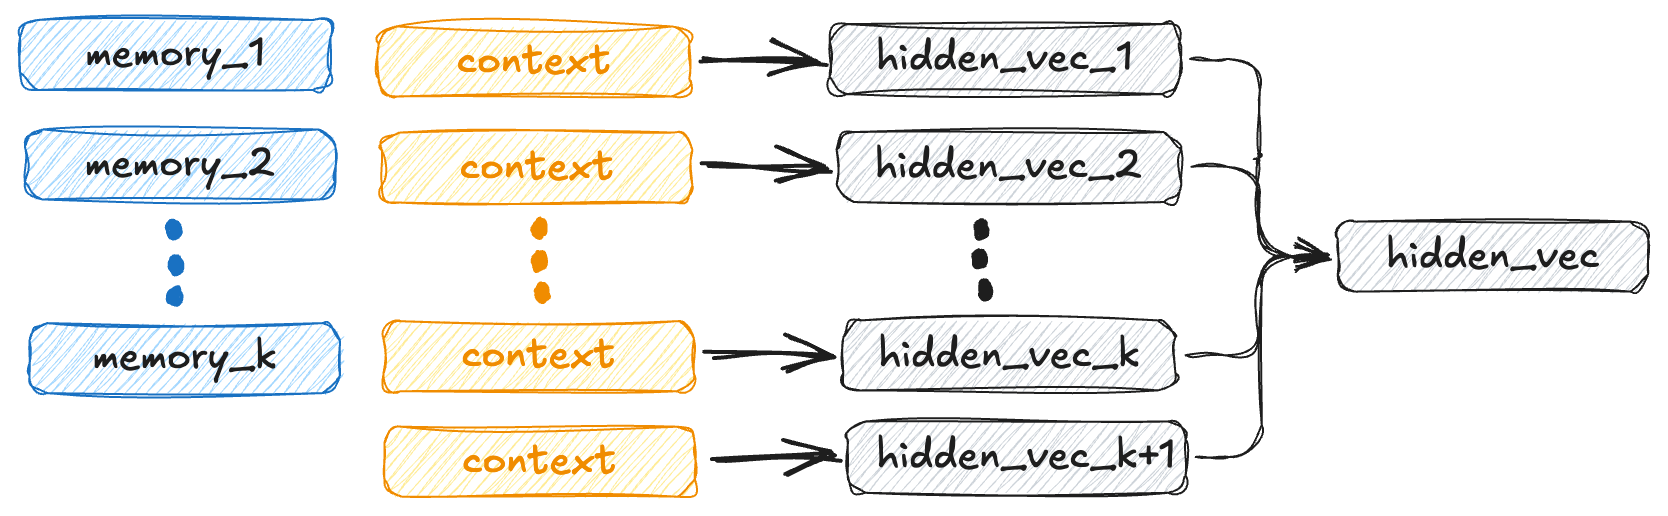
\includegraphics[width=0.7\textwidth]{figures/memory_arch.png}
    \caption{Diagram illustrating self-attention computations performed at each layer in \model. We concatenate each memory with the context (except for the last hidden vector where we only use context), apply standard self-attention and then aggregate the resulting hidden vectors to produce the final hidden vectors.}
    \label{fig:memory_arch}
\end{figure}

The working memory in \model consists of $k$ memory units, where each unit is designed to store the representations of each feedback message of $M$ tokens. 
When updating working memories, we follow the \textit{first in, first out} (FIFO) rule. 
Given refreshed text chunks of the same length from fact-checkers and retrievers, our model encodes them into the KV cache in parallel using the same positional IDs. Working memories in \model are stored as part of the language models' context preceding the model's own output text and prompts, allowing for flexible updates without reprocessing generated content. 
As shown in Figure~\ref{fig:memory_arch}, a separate embedding store is used for preserving these memories, which are then processed at each layer by concatenating them with the context. 
We then apply regular self-attention and aggregate the resulting hidden vectors using normalization terms from self-attention for each memory unit. Empirically, we find that adding hidden vectors produced by context only improves the fluency of long outputs, so we keep it in our model architectures. 
More formally, 
\begin{equation}
    \Vec{h}_n=\sum_{i=1}^{k+1}\frac{\alpha_i\Vec{h}_{n_i}}{\sum_{j=1}^{k+1}\alpha_j},
\end{equation}
\noindent where $\Vec{h}_n$ is the output vectors for self-attention at $n$-th layer in LMs, $\Vec{h}_{n_i}$ is the hidden vectors produced by memories concatenated with the context and by only the context vectors, and $\alpha_i$ is the normalization term from self-attention that leads to $\Vec{h}_{n_i}$.

